% PillCard – Portfolio-Bericht, Hands-on HCI (5,908), HSG, HS 2026
% Kompilieren in Overleaf: Compiler pdfLaTeX, Hauptdatei main.tex. Literatur in literatur.bib
% (BibLaTeX mit biber, Overleaf ruft biber automatisch auf).
% Fotos als JPG/PNG in fotos/ ablegen, Dateinamen siehe \foto{...} unten.
% Fehlt ein Foto, erscheint ein roter Platzhalter.
% Vor der Abgabe im PDF nach "OFFEN" und "PRÜFEN" suchen: Diese Stellen müssen noch geklärt werden.

\documentclass[11pt,a4paper]{article}

\usepackage[T1]{fontenc}
\usepackage[utf8]{inputenc}
\usepackage[ngerman]{babel}
\usepackage{lmodern}
\usepackage{microtype}
\usepackage[a4paper,margin=2.5cm]{geometry}
\usepackage{graphicx}
\usepackage{xcolor}
\usepackage{booktabs}
\usepackage{tabularx}
\usepackage{array}
\usepackage{enumitem}
\usepackage{caption}
\usepackage{float}
\usepackage{csquotes}
\usepackage{tikz}
\usetikzlibrary{positioning,arrows.meta,fit,backgrounds,calc}
\usepackage{listings}
\usepackage[backend=biber,style=numeric,sorting=none]{biblatex}
\addbibresource{literatur.bib}
\usepackage[hidelinks]{hyperref}

\setlength{\parindent}{0pt}
\setlength{\parskip}{0.55em}
\setlist{itemsep=0.15em,topsep=0.3em}
\captionsetup{font=small,labelfont=bf}

% Code-Ausschnitte; Umlaute in Kommentaren über literate
\lstset{
  basicstyle=\ttfamily\footnotesize,
  columns=fullflexible,
  keepspaces=true,
  frame=single,
  framerule=0.3pt,
  rulecolor=\color{black!30},
  backgroundcolor=\color{black!3},
  commentstyle=\color{black!55}\itshape,
  keywordstyle=\bfseries,
  showstringspaces=false,
  breaklines=true,
  aboveskip=0.8em,
  belowskip=0.6em,
  captionpos=b,
  literate={ä}{{\"a}}1 {ö}{{\"o}}1 {ü}{{\"u}}1 {Ä}{{\"A}}1 {Ö}{{\"O}}1 {Ü}{{\"U}}1 {ß}{{\ss}}1
}
\renewcommand{\lstlistingname}{Listing}
\renewcommand{\arraystretch}{1.2}
\newcolumntype{Y}{>{\raggedright\arraybackslash}X}

% ---------- Markierungen für den Entwurf ----------
% \offen{...}  = Information fehlt, muss das Team ergänzen
% \pruefen{...} = von uns aus Code/Doku abgeleitet, bitte bestätigen oder korrigieren
\newcommand{\offen}[1]{\textcolor{red}{\textbf{[OFFEN:} #1\textbf{]}}}
\newcommand{\pruefen}[1]{\textcolor{orange!85!black}{\textbf{[PRÜFEN:} #1\textbf{]}}}

% Code und Dateinamen
\DeclareRobustCommand{\code}[1]{\texttt{\detokenize{#1}}}

% Foto mit Platzhalter: \foto[Breite]{Dateiname in fotos/}{Wunschmotiv}
\newcommand{\foto}[3][0.8\linewidth]{%
  \IfFileExists{fotos/#2}{\includegraphics[width=#1]{fotos/#2}}{%
    \fbox{\parbox[c][4.2cm][c]{\dimexpr#1-2\fboxsep-2\fboxrule\relax}{\centering
      \textcolor{red}{\textbf{FOTO FEHLT}}\\[0.3em]
      \small Datei: \texttt{fotos/\detokenize{#2}}\\[0.2em]
      Motiv: #3}}}}

% Namen an einer Stelle pflegen
\newcommand{\maxname}{Max Jäckle}
\newcommand{\stasianame}{Anastasia \offen{Nachname}}
\newcommand{\krisname}{Kris \offen{Nachname, Schreibweise Kris/Chris}}

\title{%
  \textbf{PillCard}\\[0.4em]
  \large Ein Tablettenspender, den man nicht einstellen muss:\\
  Karte hinhalten, Becher nehmen\\[1em]
  \normalsize Portfolio-Bericht \textperiodcentered{} Hands-on HCI: Entwicklung von Software- und Hardware-Prototypen (5,908)\\
  Universität St.Gallen, Herbstsemester 2026}
\author{\maxname \and \stasianame \and \krisname}
\date{Abgabe: 20.~November 2026\\[0.5em]
  \small Code, Schaltpläne und Doku: \url{https://github.com/jmax696/PillCard}}

\begin{document}
\maketitle
\thispagestyle{empty}

\begin{abstract}
\noindent
PillCard ist ein Tablettenspender mit drei Kammern, an dem nichts eingestellt wird. Jede Person hält
ihre RFID-Karte an das Gerät und bekommt die für heute verschriebene Kombination in einen Becher.
Ein Mikrofon unter den Kammern hört, ob jede Tablette wirklich gefallen ist, und ein Kontakt aus
Kupferband merkt, ob der Becher steht und ob er abgeholt wurde. Pläne, Vorrat und Verlauf liegen auf
einem Raspberry Pi und sind über eine lokale Website einsehbar. So sieht zum Beispiel ein Enkelkind,
ob die Grossmutter ihre Tabletten heute abgeholt hat. Neue Medikamente lassen sich per QR-Code eines
Schweizer E-Rezepts einer leeren Kammer zuordnen. Der Bericht beschreibt, warum wir PillCard gebaut
haben, wie der Prototyp in einer Woche von einem Arduino-Konzept zu einem verteilten System aus
ESP32 und Raspberry Pi wurde, und was er (noch) nicht kann.
\end{abstract}

\tableofcontents
\newpage

% =====================================================================
\section{Motivation}
\label{sec:motivation}

\subsection{Problem}

Wer mehrere Medikamente nimmt, muss jeden Tag die richtige Kombination zusammenstellen und darf
weder eine Dosis vergessen noch eine doppelt nehmen. Für ältere Menschen kommt oft hinzu, dass
Angehörige nicht vor Ort sind und nur durch Nachfragen erfahren, ob alles geklappt hat.

\offen{Zahl zur Therapietreue mit echter Quelle. Vorschlag: WHO (2003), \emph{Adherence to
Long-Term Therapies: Evidence for Action}. Dort steht, dass in Industrieländern im Schnitt nur etwa
die Hälfte der Patient:innen mit Langzeittherapie ihre Medikamente wie verordnet nimmt. Vor dem
Zitieren im Original prüfen, sonst diesen Absatz weglassen.}

Elektronische Tablettenspender gibt es bereits. Nach unserer Einschätzung beim Idea Pitch müssen sie
aber am Gerät selbst programmiert werden, über kleine Displays und Tasten. Genau das ist für viele
ältere Menschen schwierig, und ein Gerät, das sich eine einzelne Person einrichtet, passt nicht zu
einem Haushalt, in dem mehrere Personen Medikamente nehmen.
\offen{Ein bis zwei konkrete Beispiele bestehender Spender mit Quelle nennen oder diesen Satz als
eigene Annahme kennzeichnen.}

Daraus entstand unsere Leitfrage:
\begin{quote}
\emph{Wie kann ein Tablettenspender aussehen, an dem die Person, die die Tabletten nimmt, gar nichts
einstellen muss, und der trotzdem mehreren Personen und ihren Angehörigen gerecht wird?}
\end{quote}

Das Projekt gehört zum Kursthema~1 \enquote{Augmenting Humans in Everyday Life}.

\subsection{Nutzer:innen und Szenarien}

Wir haben PillCard um zwei Szenarien herum entworfen. Das erste ist die Hauptgeschichte unseres Videos.

\paragraph{Oma Anna und ihr Enkelkind.}
Anna (fiktive Persona) lebt allein und nimmt täglich mehrere Tabletten. Ihr Enkelkind richtet PillCard
einmal ein: Es legt Anna als Nutzerin an, hält dabei ihre Karte an das Gerät und trägt ein, wie viele
Tabletten sie aus welcher Kammer bekommt. Anna selbst muss danach nur noch ihre Karte hinhalten und den
Becher nehmen. Ihr Enkelkind sieht auf der Website, ob Anna die Tabletten heute abgeholt hat, ob alle
herausgekommen sind und wann eine Kammer leer wird.

\paragraph{Die WG.}
In einer Wohngemeinschaft teilen sich mehrere Personen ein Gerät. Jede hat ihre eigene Karte und ihren
eigenen Plan, zum Beispiel unterschiedliche Kombinationen aus denselben drei Kammern. Das Gerät erkennt
an der Karte, wer davorsteht, und gibt jeder Person nur ihre eigene Dosis, und das nur einmal am Tag.
Unsere Test-Rezepte (Abschnitt~\ref{sec:erezept}) bilden dieses Szenario mit drei Personen ab.

\begin{table}[H]
\centering
\small
\begin{tabularx}{\linewidth}{@{}l Y Y@{}}
\toprule
\textbf{Rolle} & \textbf{Wer} & \textbf{Was die Rolle mit PillCard tut} \\
\midrule
Nutzer:in & Anna, WG-Mitglied & Karte hinhalten, Becher nehmen; optional im Nutzerbereich Verlauf ansehen und
  die Dosis nach Tagesform anpassen (nur wo erlaubt) \\
Verwaltung & Enkelkind, Angehörige, Pflege & Personen und Karten anlernen, Pläne festlegen, Kammern
  befüllen, E-Rezept scannen, Servos kalibrieren, Status aller Personen sehen \\
\bottomrule
\end{tabularx}
\caption{Rollen. Die Trennung ist der Kern des Konzepts: Alles Einstellen liegt bei der Verwaltung, am
Gerät bleibt eine einzige Handlung.}
\label{tab:rollen}
\end{table}

\subsection{Interaktionsdesign}
\label{sec:interaktion}

Die folgenden Entscheidungen prägen, wie sich PillCard für die Nutzer:innen anfühlt.

\begin{enumerate}[label=\textbf{\arabic*.}]
\item \textbf{Eine Handlung am Gerät.} Das Gerät hat keine Tasten und kein Menü. Die Karte ist
  gleichzeitig Identität und Auslöser. Alles, was Planung und Lesen erfordert, liegt auf der Website und
  damit bei den Personen, die damit umgehen können (Tabelle~\ref{tab:rollen}).
\item \textbf{Der Becher als Bestätigung.} Wer den Becher nimmt, bestätigt damit die Abholung, ohne einen
  zusätzlichen Schritt. Eine Handlung, die ohnehin nötig ist, liefert die Information für die Angehörigen.
  Umgekehrt gibt das Gerät nur aus, wenn der Becher steht, damit keine Tablette auf die Platte fällt.
\item \textbf{Schutz vor einer doppelten Dosis.} Hält jemand die Karte ein zweites Mal hin, gibt es nichts.
  Das Display zeigt \enquote{Schon genommen} und, falls hinterlegt, \enquote{Wieder um 18:00}.
\item \textbf{Mehrere Rückmeldekanäle.} Kurze Texte auf dem LCD (eine Aufforderung pro Zustand), eine
  grüne LED für \enquote{läuft/alles gut}, eine rote für \enquote{nichts ausgegeben/Problem} und das
  hörbare Klacken der fallenden Tablette.
\item \textbf{Fehler dort zeigen, wo man sie beheben kann.} Ist eine Kammer leer, leuchtet eine LED direkt
  an ihrem Einfüllstutzen. Fehlt nach der Ausgabe eine Tablette, zeigt das Display nur \enquote{Fehlt: K2 /
  App öffnen}. Die Details stehen auf der Website, weil 16~Zeichen dafür nicht reichen.
\item \textbf{Selbstbestimmung in Grenzen.} Für Kammern, die die Verwaltung freigibt (z.\,B.\ ein
  Nahrungsergänzungsmittel), kann die Person ihre Dosis für heute oder morgen selbst anpassen, aber nur bis
  zu einer festgelegten Obergrenze (\enquote{Dosis nach Tagesform}).
\item \textbf{Nachfüllen ohne Abtippen.} Eine leere Kammer belegt man neu, indem man den QR-Code des
  E-Rezepts mit dem Handy fotografiert. Die Website schlägt Medikament, Tagesmenge und Person vor.
\end{enumerate}

Tabelle~\ref{tab:display} zeigt, was das Gerät in welcher Situation anzeigt. Das LCD kann keine Umlaute,
deshalb stehen die Texte dort mit Ersatzzeichen.

\begin{table}[H]
\centering
\small
\begin{tabularx}{\linewidth}{@{}Y l l l@{}}
\toprule
\textbf{Situation} & \textbf{Zeile 1} & \textbf{Zeile 2} & \textbf{LED} \\
\midrule
Bereit (abwechselnd mit leeren Kammern) & PillCard & Karte hinhalten & -- \\
Karte erkannt, Ausgabe beginnt & Hallo Anna / Ihre Medikamente & Ausgabe startet & grün \\
Kein Becher da & Becher bitte & \textit{(Restzeit)} & -- \\
Während der Ausgabe & Kammer 1 & Tablette 1/2 & grün \\
Ausgabe fertig, Becher steht & Ihre Medikation & liegt bereit & -- \\
\quad\ldots{} und etwas fehlt (im Wechsel) & Fehlt: K2 & App öffnen & -- \\
Becher hochgenommen & Bitte einnehmen & & -- \\
Zweites Mal am selben Tag & Schon genommen & Wieder um 18:00 & rot \\
Unbekannte Karte & Karte unbekannt & App öffnen & rot \\
Becher kam nicht innerhalb von 15\,s & Kein Becher & Becher abstellen & rot \\
\bottomrule
\end{tabularx}
\caption{Zustände am Gerät (aus \code{PillCard_Demo.ino}).}
\label{tab:display}
\end{table}

\begin{figure}[H]
\centering
\foto[0.75\linewidth]{interaktion_karte.jpg}{Hand hält Karte an das Lesefeld, Display zeigt \enquote{Hallo Anna}}
\caption{Die einzige Interaktion am Gerät: Karte hinhalten.}
\end{figure}

\subsection{Was PillCard bewusst nicht kann}
\label{sec:grenzen}

Wir wollen die Funktion nicht grösser darstellen, als sie ist:
\begin{itemize}
\item \textbf{PillCard erkennt die Abholung, nicht die Einnahme.} Gemessen werden, dass die Tabletten in
  den Becher gefallen sind (Mikrofon) und dass der Becher danach hochgenommen wurde (Kupferkontakt). Ob die
  Person die Tabletten schluckt, weiss das Gerät nicht. Auf der Website steht deshalb \enquote{abgeholt},
  nicht \enquote{eingenommen}.
\item Ein voller und ein leerer Becher sehen für den Kontakt gleich aus. Wer den Becher nur kurz anhebt und
  wieder hinstellt, gilt als \enquote{abgeholt}.
\item Der Prototyp kennt eine Tagesdosis, keine Einnahmezeitpunkte. Morgens, mittags und abends aus dem
  E-Rezept werden zusammengezählt.
\item Die Website läuft nur im Heimnetz und ohne HTTPS. Das Enkelkind muss im Prototyp also im selben WLAN
  sein. Fernzugriff ist eine Erweiterung (Abschnitt~\ref{sec:erweiterungen}).
\item PillCard ist ein Studienprototyp und kein Medizinprodukt.
\end{itemize}

% =====================================================================
\section{Von der Idee zum Prototyp}
\label{sec:weg}

\subsection{Ablauf}

Tabelle~\ref{tab:ablauf} fasst die Woche zusammen. Die Zeitpunkte stammen aus dem Kursplan und aus dem
Git-Verlauf des Repos.

\begin{table}[H]
\centering
\small
\begin{tabularx}{\linewidth}{@{}l Y@{}}
\toprule
\textbf{Tag} & \textbf{Was passiert ist} \\
\midrule
Mo 26.10. & Kurs-Einführung, Projektidee. Wir übernehmen den Magazin- und Schiebermechanismus aus
  DoseMinder~\cite{doseminder} als Vorlage und planen in FreeCAD eine Grundplatte (\enquote{Base}) für
  drei Module sowie eine Rinne, die alle drei Kammern in einen Becher leitet. \\
Di 27.10. & \textbf{Idea Pitch}. Erstes Konzept in \code{README.md} und \code{REQUIREMENTS.md}: Arduino Uno,
  Plan auf der RFID-Karte gespeichert, je eine Lichtschranke pro Kammer, Mikrofon als Plan~B. Druckteile
  für drei Module vorbereitet. \\
Mi 28.10. & Bauteile einzeln getestet (Servo, LCD, RFID). Umstieg auf ESP32, dann Aufteilung: ESP32 für
  Servos/Display/Sensoren, Raspberry Pi für RFID, Datenbank und Website. Mikrofon-Prüfung im
  Demo-Sketch, SQLite-Datenbank, erste lokale Website mit Anlernen per Scan und Kalender. \\
Do 29.10. & Neue 3D-Version der Kammern (Servos starten von der anderen Seite), Demo-Dashboard,
  Leer-LEDs an den Einfüllstutzen, E-Rezept-Scan. \textbf{Prototype Demo} um 16~Uhr. \\
Fr 30.10. & Becherkontakt aus Kupferband, Abholanzeige und Servo-Kalibrierung auf der Website,
  Fehlt-Meldung in der App, A4-Testrezept. \textbf{Video Showcase} um 16~Uhr. \\
bis 20.11. & Aufräumen, Video, Bericht. \offen{Was wurde nach dem 30.10. noch gebaut oder geändert,
  z.\,B.\ am Gehäuse?} \\
\bottomrule
\end{tabularx}
\caption{Ablauf der Projektwoche.}
\label{tab:ablauf}
\end{table}

\begin{figure}[H]
\centering
\foto[0.48\linewidth]{prozess_skizze.jpg}{erste Skizze oder Pitch-Folie}\hfill
\foto[0.48\linewidth]{prozess_breadboard.jpg}{Breadboard mit ESP32, Servo und LCD beim Einzeltest}
\caption{Zwischenstände: erste Idee und erster Aufbau auf dem Breadboard.}
\end{figure}

\subsection{Sechs Entscheidungen, die den Prototyp geprägt haben}
\label{sec:entscheidungen}

Der fertige Prototyp unterscheidet sich deutlich vom Konzept des Idea Pitch. Tabelle~\ref{tab:entscheidungen}
zeigt, was sich geändert hat und warum. Die Abschnitte~\ref{sec:umsetzung} und~\ref{sec:reflexion} gehen auf
die Details ein.

\begin{table}[H]
\centering
\small
\begin{tabularx}{\linewidth}{@{}>{\raggedright\arraybackslash}p{2.6cm} Y Y Y@{}}
\toprule
\textbf{Thema} & \textbf{Geplant (27.10.)} & \textbf{Umgesetzt} & \textbf{Warum} \\
\midrule
Steuerung & Arduino Uno für alles & ESP32 für Servos, Display, LEDs, Mikrofon und Becher; Raspberry Pi für
  RFID, Daten und Website, verbunden über ein USB-Kabel &
  Der RC522 lief am Uno nie (Firmware-Version 0x00). Die Pins des Uno reichen nicht für ein LCD ohne
  I²C-Modul plus Servos, Sensoren und LEDs. Eine Website mit Datenbank braucht einen Rechner. \\
Wo der Plan liegt & Auf der RFID-Karte (eigenes 48-Byte-Format mit Prüfsumme) & In einer SQLite-Datenbank
  auf dem Pi; die Karte ist nur noch eine ID &
  Das Beschreiben der Karten hat nie funktioniert. Mit der Datenbank lassen sich Pläne ändern, ohne die
  Karte neu zu beschreiben, und jede Ausgabe wird für die Angehörigen protokolliert.
  \pruefen{Begründung so richtig?} \\
Zählen der Tabletten & Drei Lichtschranken, eine pro Kammer & Ein Mikrofon unter allen Kammern &
  Ein Sensor statt drei. Weil die Kammern nacheinander ausgeben, ist trotzdem klar, aus welcher Kammer
  eine Tablette kam. \pruefen{Gab es weitere Gründe, z.\,B.\ Platz oder fehlende Lichtschranken?} \\
Becher erkennen & Kontaktsensor, Details offen & Zwei Kupferflächen auf der Grundplatte, Kupferband
  unter dem Becher verbindet sie & Billig, flach, keine Mechanik. Liefert zwei Informationen: Becher steht
  (Ausgabe erlaubt) und Becher genommen (abgeholt). \\
Neues Medikament & Kamera am Gerät liest den QR-Code & Handykamera im Browser oder USB-Scanner auf der
  Verwaltungsseite & Keine zusätzliche Hardware am Gerät. Eine Live-Kamera im Browser geht ohne HTTPS
  nicht, ein Foto schon. \\
Servo-Winkel & Fest im Code, Kalibrieren über den Seriellen Monitor & Einstellbar auf der Website,
  gespeichert in der Datenbank & Nach der neuen 3D-Version stimmten alle Winkel nicht mehr. Über die Website
  geht das Einstellen ohne Laptop und ohne den ESP32 neu zu flashen. \\
\bottomrule
\end{tabularx}
\caption{Entscheidungen vom Konzept zum Prototyp.}
\label{tab:entscheidungen}
\end{table}

% =====================================================================
\section{Umsetzung}
\label{sec:umsetzung}

\subsection{Systemüberblick}

PillCard besteht aus zwei Rechnern mit klarer Aufgabenteilung (Abbildung~\ref{fig:system}). Der
\textbf{Raspberry Pi} entscheidet, wer was bekommt. Er liest die Karte, schlägt den Plan in der Datenbank
nach, prüft, ob heute schon ausgegeben wurde, und betreibt die Website. Der \textbf{ESP32} führt aus. Er
fährt die Servos, hört mit dem Mikrofon mit, prüft den Becher und zeigt alles auf Display und LEDs. Die
beiden sprechen über ein USB-Kabel, das den ESP32 auch mit Strom versorgt, in einfachen Textzeilen.

\begin{figure}[H]
\centering
\resizebox{\linewidth}{!}{%
\begin{tikzpicture}[
  font=\small,
  box/.style={draw, rounded corners=2pt, align=center, minimum height=0.9cm, inner sep=4pt, fill=white},
  grp/.style={draw, dashed, rounded corners=4pt, inner sep=7pt},
  arr/.style={-{Stealth[length=2mm]}, thick},
  both/.style={{Stealth[length=2mm]}-{Stealth[length=2mm]}, thick}]
  % Pi
  \node[box] (rfid) {RFID-Leser\\RC522};
  \node[box, right=1.1cm of rfid] (pc) {\texttt{pillcard.py}};
  \node[box, below=0.7cm of pc] (db) {SQLite\\\texttt{pillcard.db}};
  \node[box, right=1.1cm of db] (web) {\texttt{web.py}\\(Flask)};
  \node[grp, fit=(rfid)(pc)(db)(web), label={[font=\small\bfseries]above:Raspberry Pi}] (pi) {};
  % Karte und Browser
  \node[box, left=1.0cm of rfid] (karte) {RFID-Karte\\der Person};
  \node[box, below=1.2cm of web] (browser) {Browser\\(Handy, Laptop)\\im Heimnetz};
  % ESP32
  \node[box, anchor=west, minimum width=2.6cm] (esp) at ($(pi.east |- pc)+(1.4cm,0)$) {\textbf{ESP32}\\\texttt{PillCard\_Demo.ino}};
  \node[box, right=1.0cm of esp, yshift=1.3cm] (servo) {3 Servos\\(Kammern)};
  \node[box, right=1.0cm of esp] (lcd) {LCD 16$\times$2,\\LEDs};
  \node[box, right=1.0cm of esp, yshift=-1.3cm] (mic) {Mikrofon,\\Becherkontakt};
  % Pfeile
  \draw[arr] (karte) -- (rfid);
  \draw[arr] (rfid) -- node[above]{SPI} (pc);
  \draw[both] (pc) -- (db);
  \draw[both] (db) -- (web);
  \draw[both] (web) -- node[right]{HTTP} (browser);
  \draw[both] (pc) -- node[above]{USB} node[below,font=\scriptsize]{Textzeilen} (esp);
  \draw[arr] (esp) -- (servo);
  \draw[arr] (esp) -- (lcd);
  \draw[arr] (mic) -- (esp);
\end{tikzpicture}}
\caption{Aufbau von PillCard. Der Pi entscheidet, der ESP32 führt aus.}
\label{fig:system}
\end{figure}

Eine Ausgabe läuft so ab:
\begin{enumerate}
\item Die Person hält ihre Karte an den Leser. \code{pillcard.py} liest die UID und ignoriert dieselbe Karte
  danach 3\,s lang.
\item Der Pi sucht die Person. Unbekannte Karte: \code{MELDUNG unbekannt}. Heute schon ausgegeben:
  \code{MELDUNG schon_genommen 18:00}. Sonst berechnet er die heutige Dosis (Plan plus eventuelle Anpassung)
  und schickt einen Auftrag, z.\,B.\ \code{AUFTRAG 17 K1=1 K3=2}.
\item Der ESP32 wartet bis zu 15\,s auf den Becher, gibt dann Kammer für Kammer jede Tablette einzeln aus und
  meldet nach jeder \code{TABLETTE 17 K1 ok} oder \code{... fehlt}, am Ende \code{FERTIG 17 K1=1 K3=2}.
\item Der Pi trägt Bestelltes und laut Mikrofon Erhaltenes in die Datenbank ein, auch bei Fehlern, damit nichts
  doppelt ausgegeben wird.
\item Wird der Becher später hochgenommen, meldet der ESP32 \code{BECHER 17 genommen 3} (vor 3\,s
  hochgenommen). Der Pi trägt die Zeit der Abholung nach. Ab jetzt zeigt die Website \enquote{abgeholt}.
\end{enumerate}

\begin{figure}[H]
\centering
\foto[0.85\linewidth]{prototyp_gesamt.jpg}{fertiger Prototyp von vorne: drei Kammern, Display, Becher, Lesefeld}
\caption{Der fertige Prototyp.}
\label{fig:prototyp}
\end{figure}

\subsection{Mechanik und Gehäuse}
\label{sec:mechanik}

\paragraph{Ausgabemechanismus.}
Für das Vereinzeln der Tabletten haben wir das Rad nicht neu erfunden. Magazin, Schieber, Servohalter und
Rampe stammen aus dem Projekt \emph{DoseMinder} von mariddc~\cite{doseminder}, einem Abschlussprojekt an der
Universität São Paulo. Die Tabletten liegen gestapelt im Magazin, ein Micro-Servo (SG90) bewegt einen
Schieber, der die unterste Tablette seitlich auf die Rampe drückt. Das Original hat einen Spender für eine
Sorte. Wir brauchten drei.

\paragraph{Eigene Teile.}
Darauf aufbauend haben wir in FreeCAD eigene Teile entworfen:
\begin{itemize}
\item eine \textbf{Grundplatte} (\enquote{Base}, 195\,$\times$\,61\,mm) mit drei Taschen, in die die Servohalter
  im Abstand von 65\,mm gesteckt werden, mit Kabellöchern und einem Durchlass für ESP32 und USB;
\item eine \textbf{Rinne} mit V-Boden (26,6° Gefälle, dieselbe Neigung wie die DoseMinder-Rampe), die die
  Tabletten aller drei Rampen zu einem Auslass in der Mitte leitet, unter dem der Becher steht
  (Abbildung~\ref{fig:cad}). Dafür ist die Base in Version~2 30\,mm höher (100\,mm), damit ein Becher bis
  55\,mm Durchmesser und 50\,mm Höhe darunter passt.
\end{itemize}
Am 29.10. kam eine neue 3D-Version der Kammern hinzu, bei der die Servos aus der anderen Richtung
anfahren. \pruefen{Was genau wurde an der 3D-Version geändert, und von wem?}
\offen{Ob Base und Rinne genau so gedruckt und verbaut wurden oder ob das Gehäuse von Kris sie ersetzt hat.}

\begin{figure}[H]
\centering
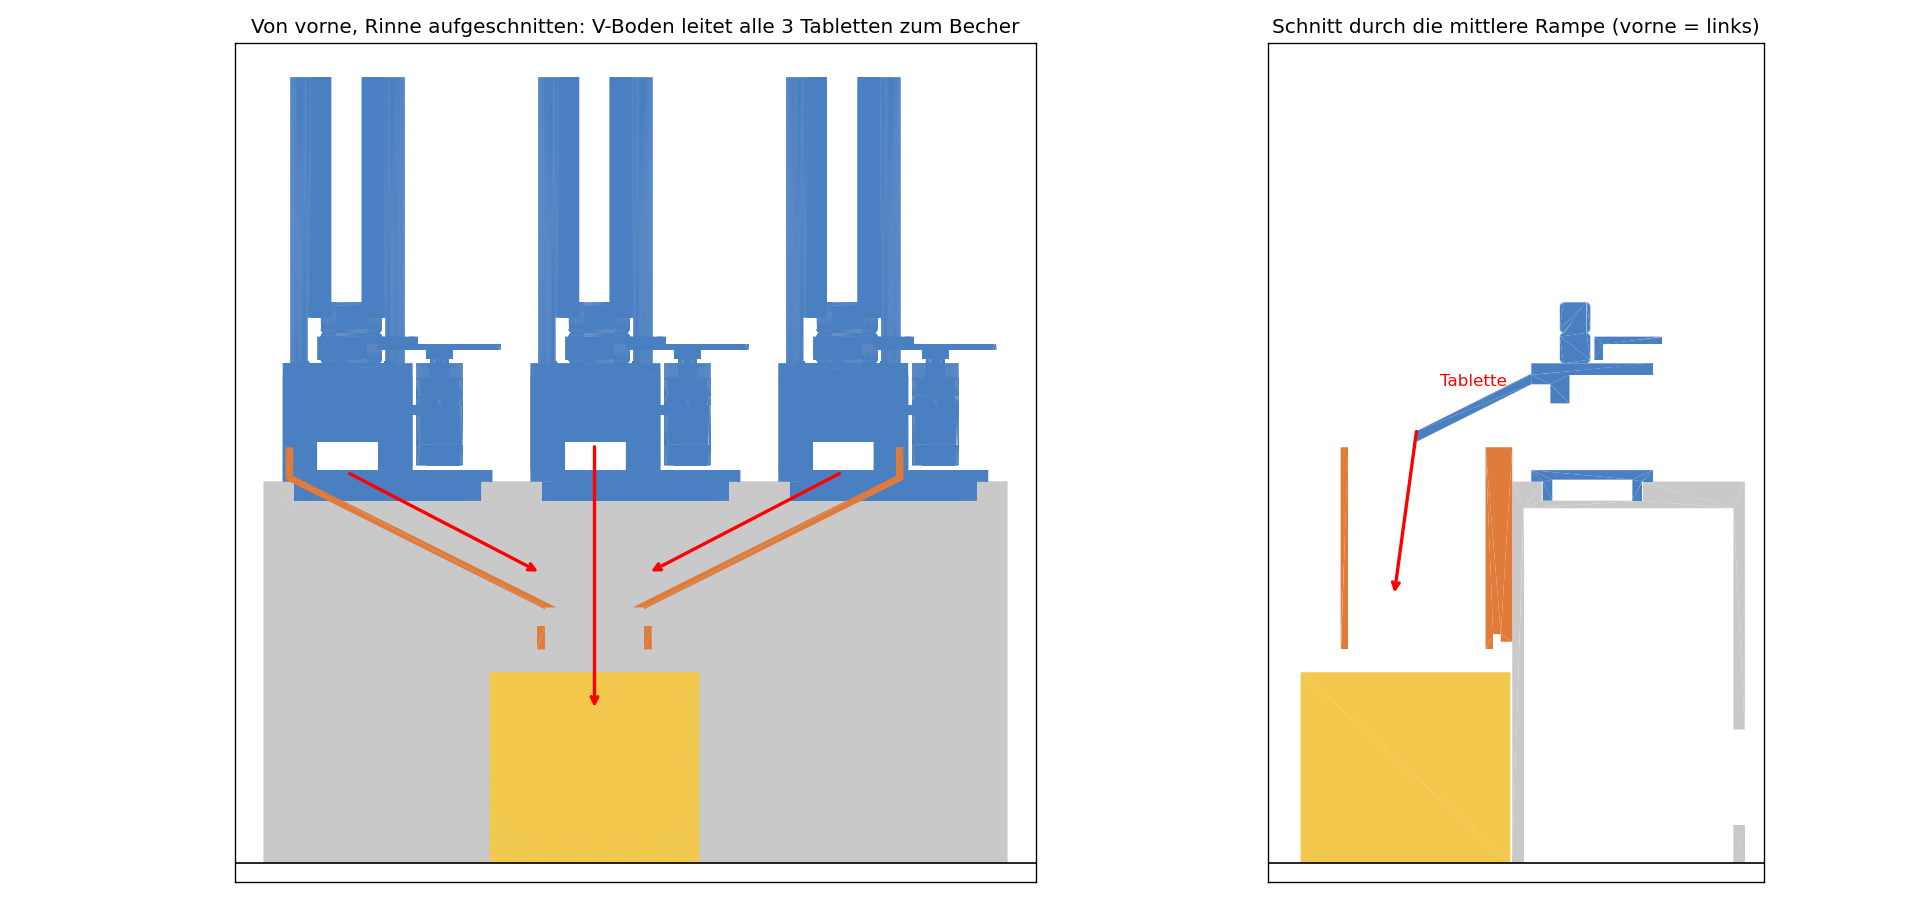
\includegraphics[width=\linewidth]{abbildungen/CAD_Rinne_Vorschau.png}
\caption{Planung vom 26.10.: drei DoseMinder-Module auf der Base, die Rinne (orange) leitet alle Tabletten
in einen Becher (gelb). Rechts ein Schnitt durch die mittlere Rampe.}
\label{fig:cad}
\end{figure}

\begin{figure}[H]
\centering
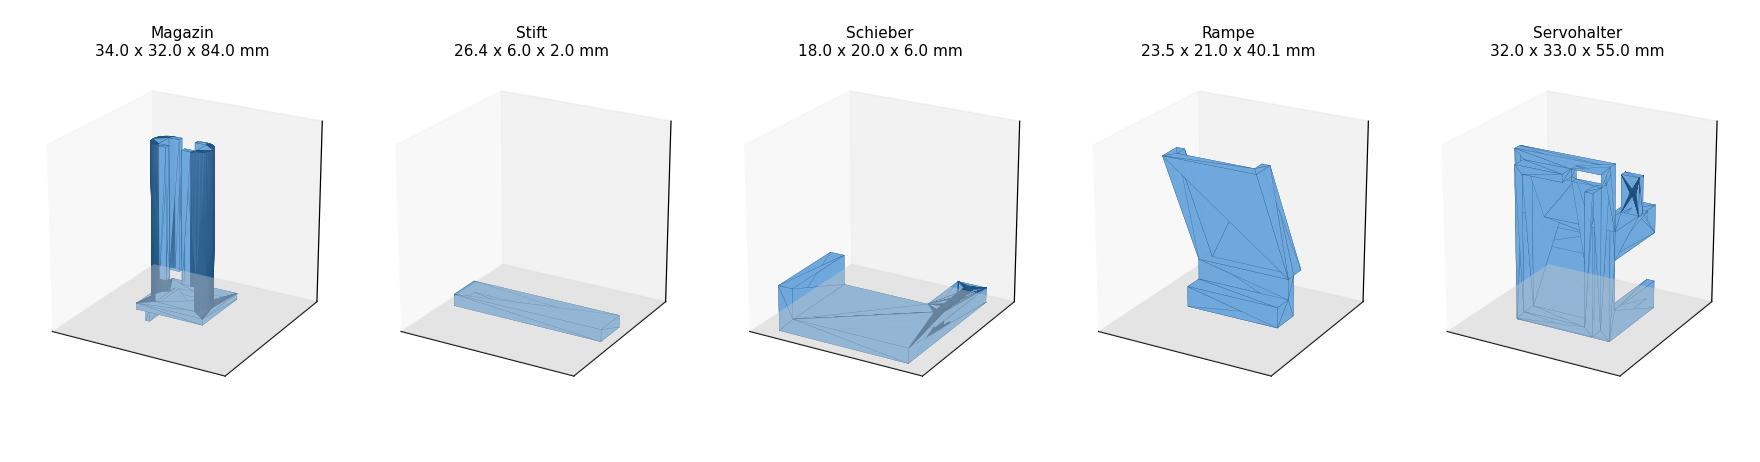
\includegraphics[width=0.6\linewidth]{abbildungen/CAD_Drucklage.png}
\caption{Druckteile eines Moduls in Drucklage: Magazin, Stift, Schieber, Rampe, Servohalter.}
\end{figure}

\paragraph{Gehäuse.}
\offen{Gehäuse von Kris beschreiben: Material (3D-Druck, Laser-Cut-MDF?), Masse, wo Display, LEDs, Lesefeld
und Becher sitzen, warum so. Mit Foto.}

\begin{figure}[H]
\centering
\foto[0.48\linewidth]{mechanik_kammer.jpg}{eine Kammer offen: Magazin, Schieber, Servo}\hfill
\foto[0.48\linewidth]{gehaeuse_innen.jpg}{Gehäuse von innen mit Verkabelung}
\caption{Mechanik und Gehäuse.}
\end{figure}

\subsection{Elektronik}
\label{sec:elektronik}

Tabelle~\ref{tab:bauteile} listet die Bauteile. Die vollständige Pinbelegung steht in
Anhang~\ref{sec:pins}, die Schaltpläne in Abbildung~\ref{fig:schaltplan-esp} und~\ref{fig:schaltplan-pi}.

\begin{table}[H]
\centering
\small
\begin{tabularx}{\linewidth}{@{}l c Y@{}}
\toprule
\textbf{Bauteil} & \textbf{Anz.} & \textbf{Wofür und warum dieses} \\
\midrule
ESP32-WROOM (Keyestudio) & 1 & Steuert die Aktoren und liest die Sensoren. Genug Pins für ein LCD ohne I²C,
  ADC für das Mikrofon, PWM für drei Servos. \\
Raspberry Pi \offen{Modell} & 1 & Liest die Karten, hält die Datenbank, betreibt die Website. \\
RFID-Leser RC522 + MIFARE-Karten & 1 & Identifiziert die Person. Hängt per SPI am Pi. \\
Micro-Servo SG90 & 3 & Je einer pro Kammer, bewegt den Schieber. \\
LCD 16$\times$2 (ohne I²C) + Poti 10\,k$\Omega$ & 1 & Textanzeige im 4-Bit-Modus, Poti für den Kontrast. \\
LEDs grün/rot & 2 & Status: Ausgabe läuft bzw.\ keine Ausgabe/Problem. \\
LEDs am Einfüllstutzen & 3 & Leuchten, wenn eine Kammer leer ist. \\
Mikrofonmodul (analog) & 1 & Hört fallende Tabletten. Liegt unter allen Kammern, ersetzt die Lichtschranken. \\
Kupferband, 1\,k$\Omega$, 10\,k$\Omega$, 100\,nF & -- & Becherkontakt mit Pull-up und Filter. \\
Breadboard-Netzteilmodul (Elegoo) & 1 & Eigene 5\,V für Servos und LCD. \\
\bottomrule
\end{tabularx}
\caption{Bauteile.}
\label{tab:bauteile}
\end{table}

\paragraph{Stromversorgung.}
Ein SG90 zieht beim Anlaufen bis zu etwa 650\,mA, ein USB-Port liefert 500\,mA. Hängen mehrere Servos am
5-V-Pin des Mikrocontrollers, bricht die Spannung ein und der Controller oder der RFID-Leser startet neu.
Servos und LCD hängen deshalb am separaten Netzteilmodul. Nur GND ist mit dem ESP32 verbunden, das Plus
des Moduls nie. Der Pi hat ein eigenes Netzteil und versorgt den ESP32 über das USB-Kabel mit.

\paragraph{Pegel.}
Der ESP32 und der Pi vertragen an ihren Pins nur 3,3\,V. Deshalb liegt R/W des LCD fest an GND (sonst könnte
das Display 5\,V auf die Datenleitungen legen), das Mikrofon läuft an 3,3\,V statt 5\,V, und der RC522 hängt
an 3,3\,V des Pi.

\paragraph{Becherkontakt.}
Auf der Grundplatte liegen zwei Kupferflächen, ein äusserer Ring an GND und eine innere Fläche über
1\,k$\Omega$ an IO13. Ein 10-k$\Omega$-Widerstand zieht IO13 auf 3,3\,V, ein 100-nF-Kondensator nach GND glättet
Störungen. Unter dem Becher klebt Kupferband. Steht der Becher, verbindet es beide Flächen und IO13 geht
auf LOW.

\begin{figure}[p]
\centering
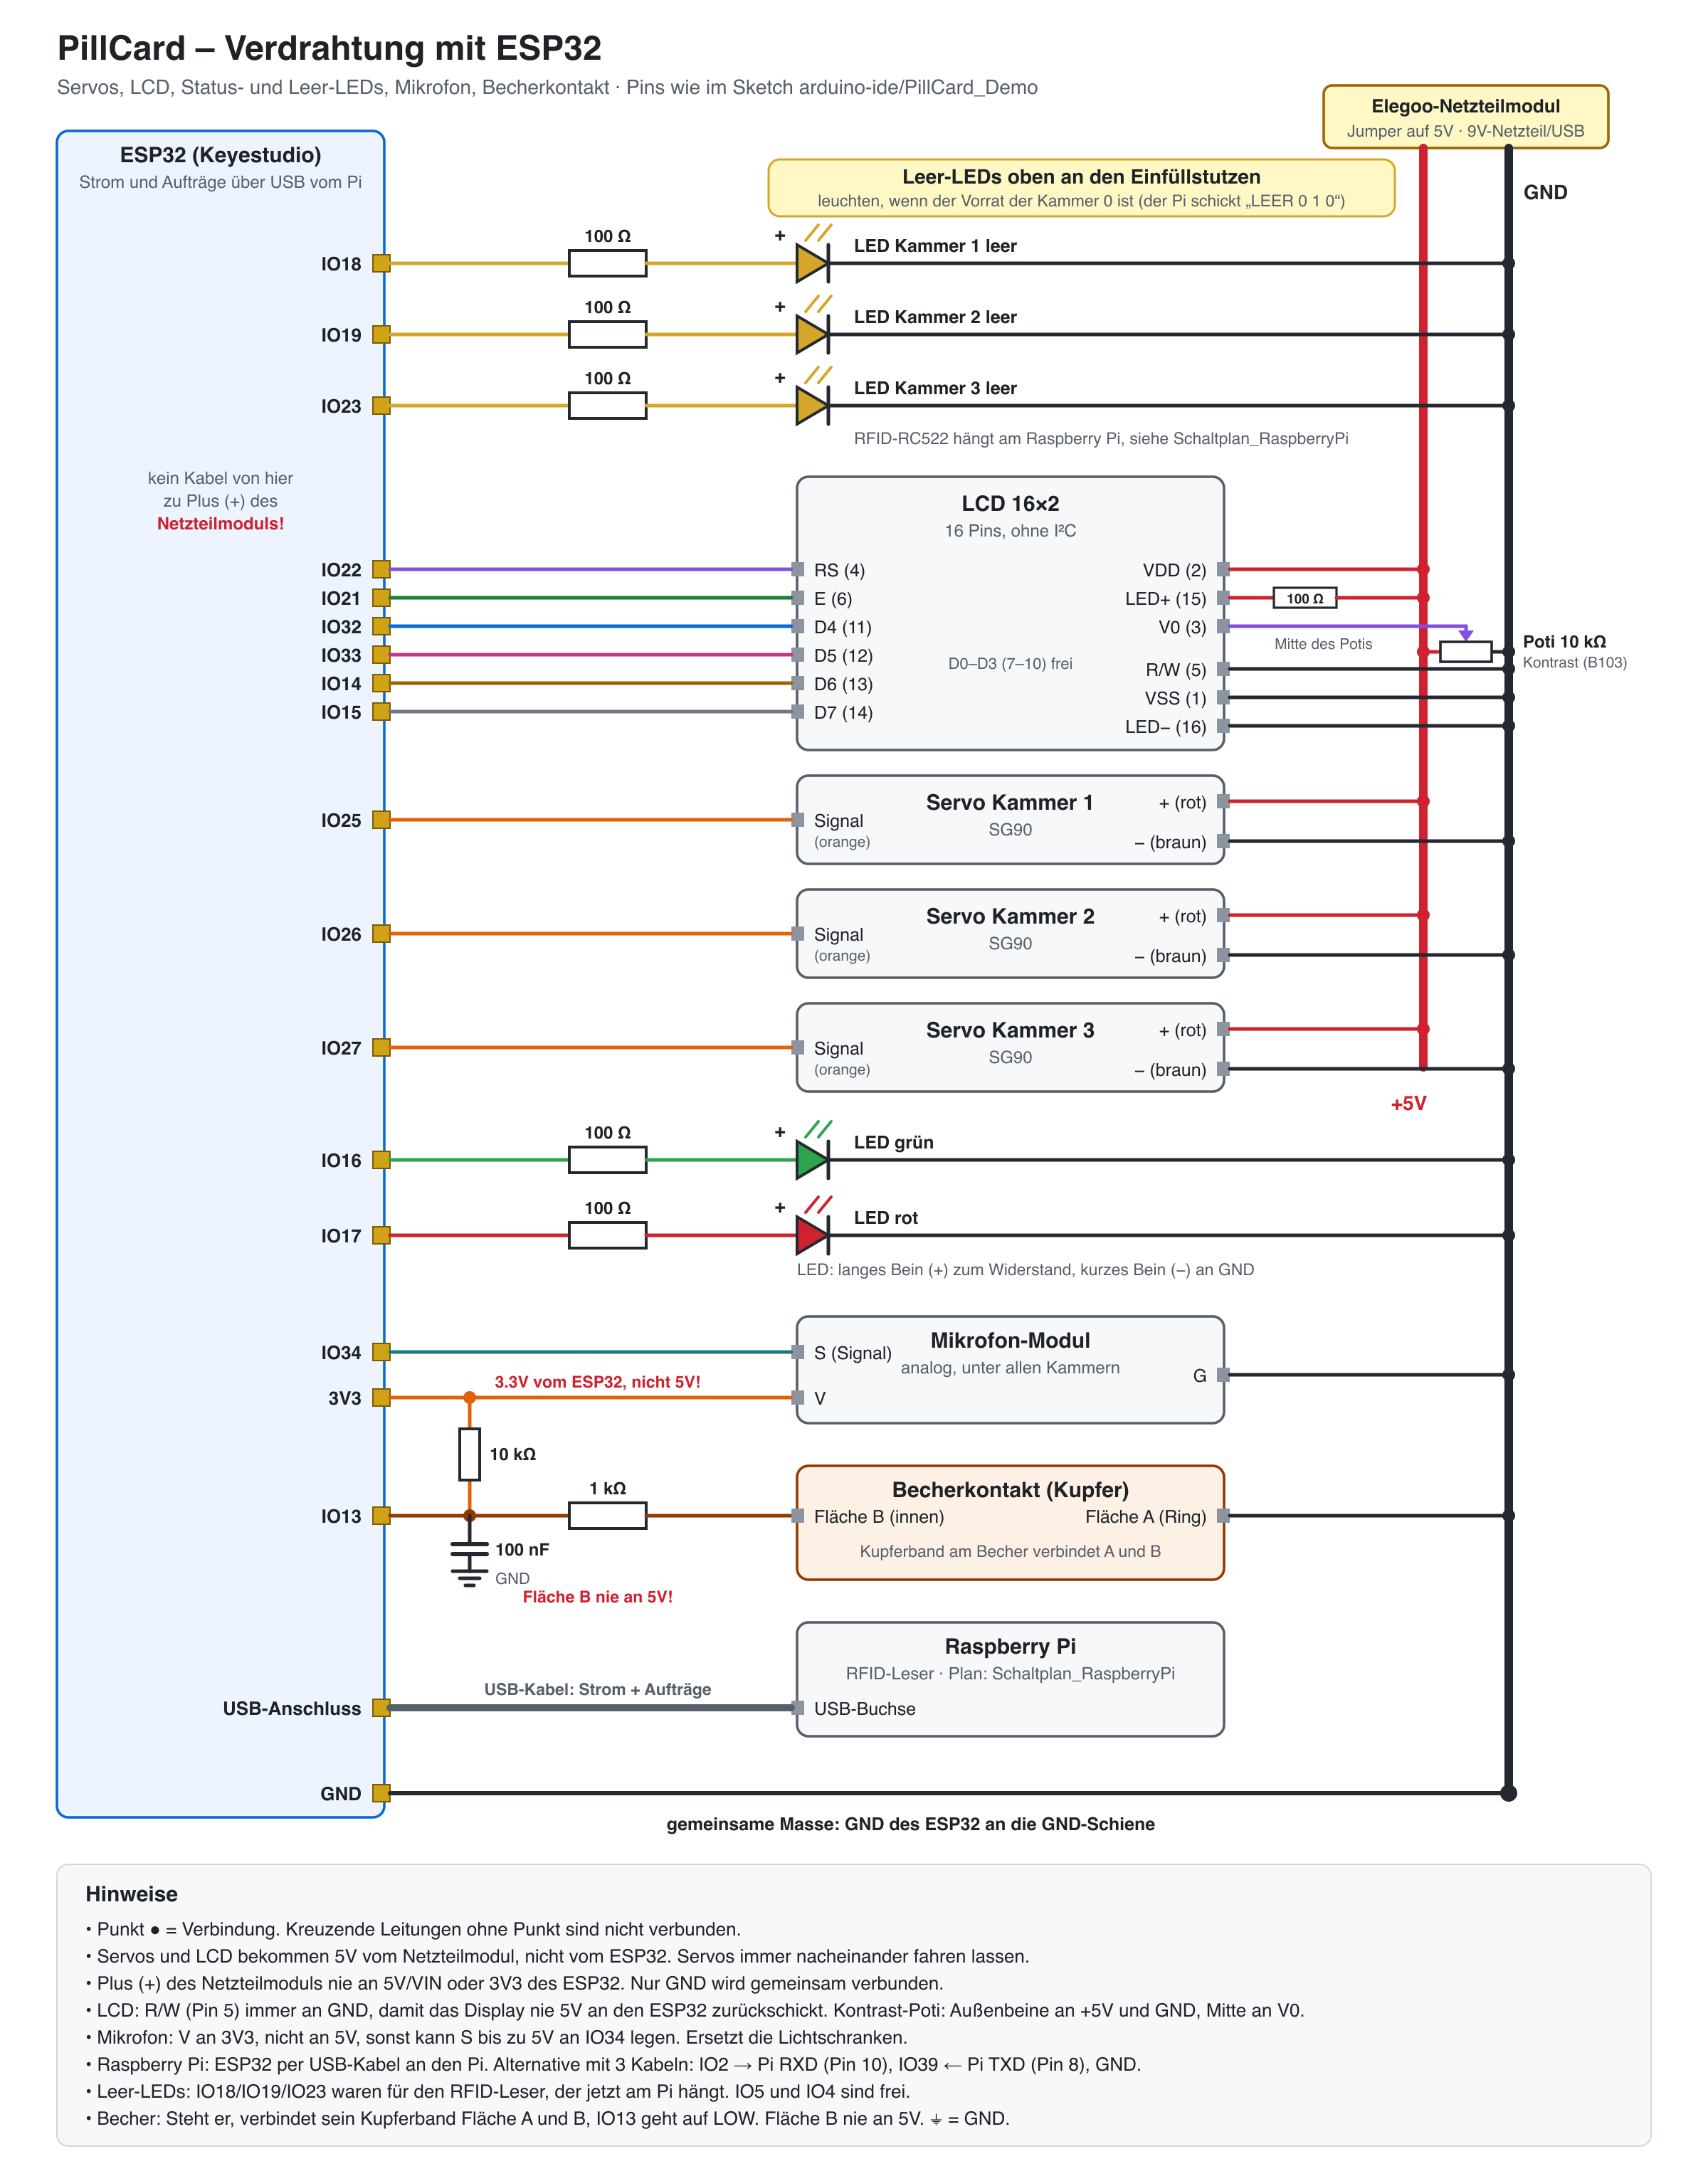
\includegraphics[width=\linewidth,height=0.85\textheight,keepaspectratio]{abbildungen/Schaltplan_ESP32.png}
\caption{Schaltplan ESP32: LCD mit Kontrast-Poti, drei Servos, Status- und Leer-LEDs, Mikrofon, Becherkontakt
an IO13, Netzteilmodul. Quelle: \code{docs/Schaltplan_ESP32.svg}.}
\label{fig:schaltplan-esp}
\end{figure}

\begin{figure}[H]
\centering
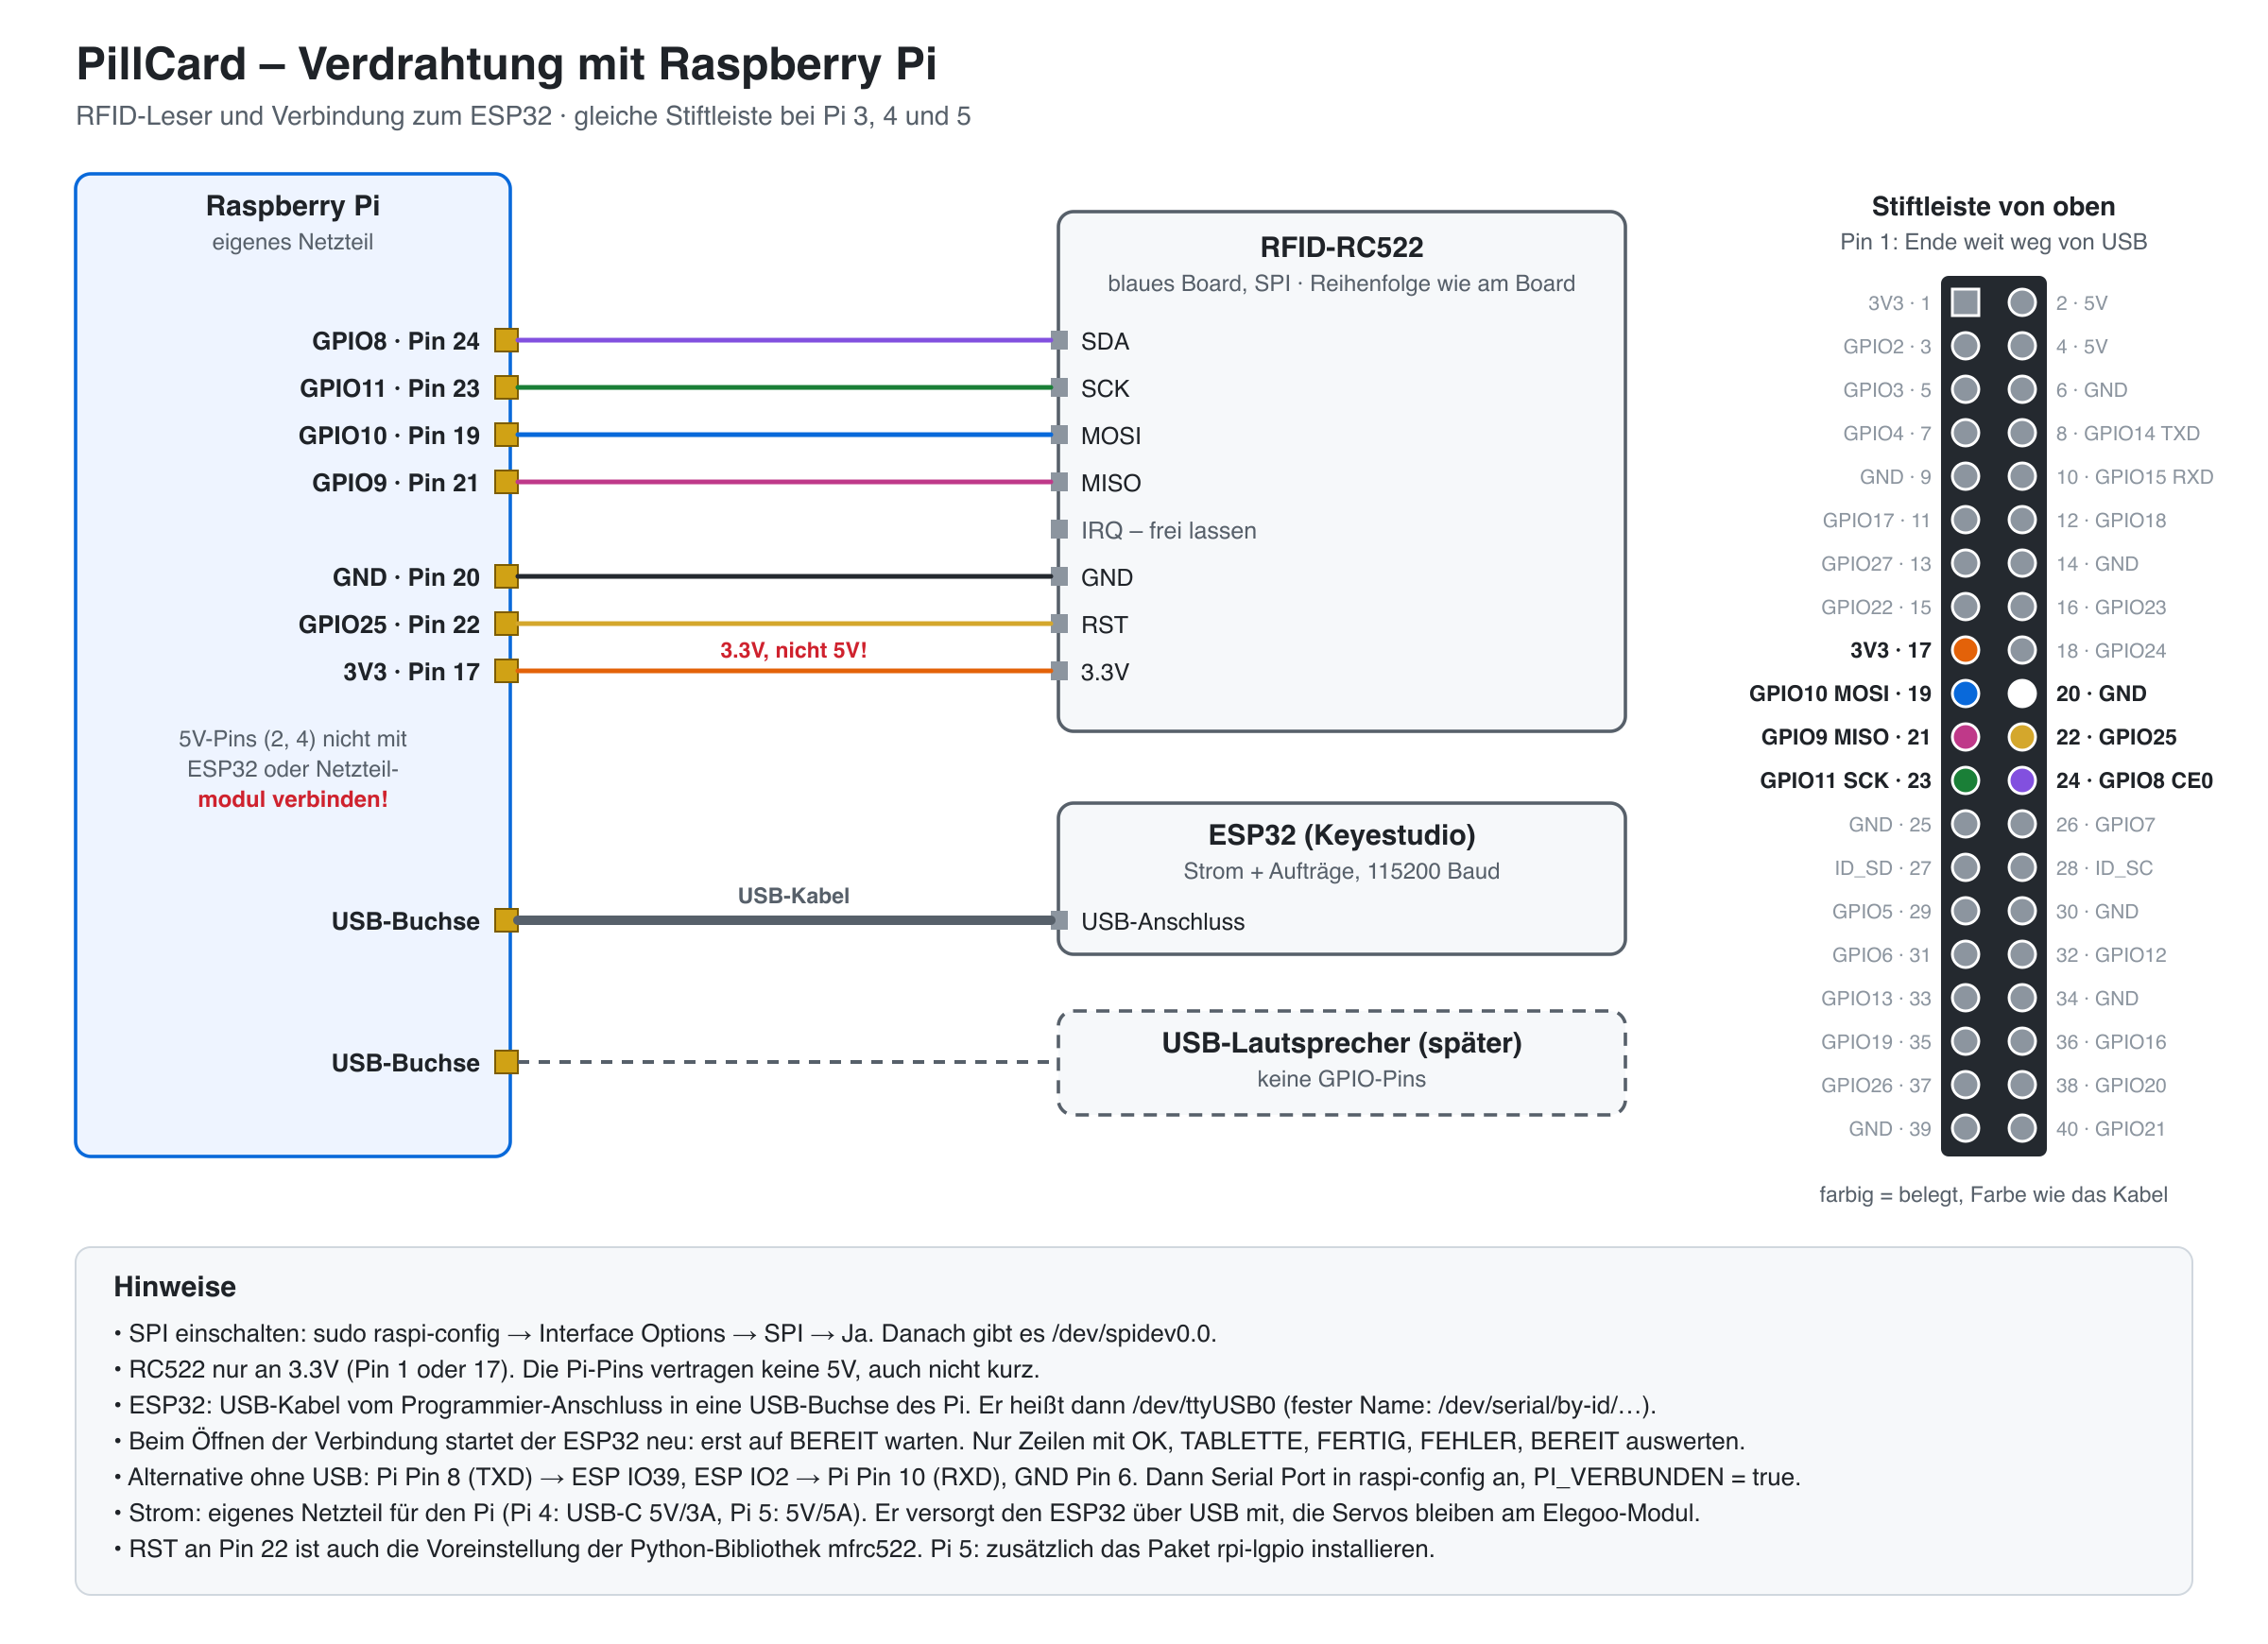
\includegraphics[width=\linewidth,height=0.6\textheight,keepaspectratio]{abbildungen/Schaltplan_RaspberryPi.png}
\caption{Schaltplan Raspberry Pi: RC522 an SPI0, ESP32 per USB. Quelle: \code{docs/Schaltplan_RaspberryPi.svg}.}
\label{fig:schaltplan-pi}
\end{figure}

\begin{figure}[H]
\centering
\foto[0.48\linewidth]{becher_kupfer.jpg}{Grundplatte mit den zwei Kupferflächen und Becher mit Kupferband}\hfill
\foto[0.48\linewidth]{mikrofon.jpg}{Mikrofonmodul unter den Kammern}
\caption{Die beiden Sensoren, die prüfen, was wirklich passiert ist.}
\end{figure}

\subsection{Software auf dem ESP32}
\label{sec:esp}

Der Sketch \code{arduino-ide/PillCard_Demo/PillCard_Demo.ino} (Arduino IDE, Board \enquote{ESP32 Dev
Module}) nimmt Textzeilen über USB entgegen und antwortet ebenso. Dasselbe Protokoll kann man im Seriellen
Monitor von Hand tippen, so liess sich der ESP32 ohne Pi testen. Tabelle~\ref{tab:protokoll} zeigt die
wichtigsten Zeilen.

\begin{table}[H]
\centering
\small
\begin{tabularx}{\linewidth}{@{}l Y@{}}
\toprule
\textbf{Zeile} & \textbf{Bedeutung} \\
\midrule
\multicolumn{2}{@{}l}{\textit{Pi $\rightarrow$ ESP32}} \\
\code{AUFTRAG 17 K1=1 K3=2} & Auftrag 17: eine Tablette aus Kammer 1, zwei aus Kammer 3 \\
\code{MELDUNG schon_genommen 18:00} & Hinweis aufs Display \\
\code{LEER 0 1 0} & Leer-LEDs: Kammer 2 ist leer \\
\code{WINKEL 170 80 170 80 10 100} & Ruhe- und Ausgabewinkel je Kammer (nach dem Kalibrieren) \\
\code{servo 3 12}, \code{probe 3} & Kalibrieren: Servo auf Winkel stellen bzw.\ Probe-Ausgabe \\
\midrule
\multicolumn{2}{@{}l}{\textit{ESP32 $\rightarrow$ Pi}} \\
\code{BEREIT} & ESP32 ist (neu) gestartet \\
\code{OK 17}, \code{TABLETTE 17 K1 ok} & Auftrag angenommen, Tablette gehört bzw.\ \code{fehlt} \\
\code{FERTIG 17 K1=1 K3=1} & Ergebnis laut Mikrofon \\
\code{FEHLER kein_becher} & Becher kam nicht, nichts ausgegeben \\
\code{BECHER 17 genommen 3} & Becher vor 3\,s hochgenommen \\
\code{BECHER 17 abgebrochen} & Becher mitten in der Ausgabe weggenommen \\
\bottomrule
\end{tabularx}
\caption{Textprotokoll zwischen Pi und ESP32 (115200~Baud).}
\label{tab:protokoll}
\end{table}

\paragraph{Ausgabe einer Tablette.}
Vor jeder Tablette fährt der Servo in die Ruhelage, dann in die Ausgabeposition und zurück. Ein SG90 hat ohne
Steuerpulse keine Haltekraft, Reibung und Tabletten würden ihn verdrehen. Deshalb bleiben die Servos
dauerhaft angesteuert. Die Winkel liegen nie bei genau 0° oder 180°, weil ein SG90 dort gegen seinen
Anschlag drückt und brummt. Kammer~3 fährt langsamer (800\,ms), weil sie sonst zu ruckartig ausgibt.

\paragraph{Zählen mit dem Mikrofon.}
Ab dem Servo-Befehl misst der ESP32 in Stücken von 50\,ms den Spitze-Spitze-Pegel des Mikrofons (ADC,
0--4095), insgesamt Fahrzeit plus 1800\,ms. Das Fenster ist so lang, weil Tabletten aus Kammer~2 und~3 oft
erst nach 0,8--1\,s fallen. Die ersten 150\,ms zählen nicht, da ist vor allem der Servo laut. Liegt der
lauteste Pegel über der Schwelle von 200 (Grundrauschen etwa 110--150), gilt die Tablette als gefallen. Einen
zweiten Versuch gibt es bewusst nicht: Überhört das Mikrofon eine Tablette, die doch gefallen ist, käme beim
zweiten Versuch eine zu viel. Lieber meldet PillCard \enquote{fehlt}, und ein Mensch sieht nach. Für das
Einstellen gibt es die Befehle \code{mikro} (Pegel 10\,s live) und \code{probe 2} (Pegelverlauf einer
Ausgabe).

\begin{lstlisting}[language=C++,caption={Kern der Mikrofonprüfung, gekürzt aus \texttt{hinhoeren()} in \texttt{arduino-ide/PillCard\_Demo/PillCard\_Demo.ino} (Servo-Ansteuerung und Ausgaben weggelassen).},label={lst:mikro}]
for (uint16_t ab = 0; ab < fenster; ab += MIC_STUECK_MS) {   // Stücke von 50 ms
  int tief = 4095, hoch = 0;
  while (millis() - start < (unsigned long)(ab + MIC_STUECK_MS)) {
    int wert = analogRead(PIN_MIKRO);
    if (wert < tief) tief = wert;
    if (wert > hoch) hoch = wert;
  }
  int pegel = hoch - tief;                  // Spitze-Spitze in diesem Stück
  bool zaehlt = ab >= MIC_IGNORIEREN_MS;    // die ersten 150 ms ist der Servo laut
  if (zaehlt && pegel > lautester) lautester = pegel;
}
return lautester;   // >= MIC_SCHWELLE (200): Tablette gefallen
\end{lstlisting}

\paragraph{Becherlogik.}
Der Kontakt wird entprellt: 50\,ms durchgehend geschlossen heisst \enquote{Becher steht}, 400\,ms offen heisst
\enquote{weg}, damit eine fallende Tablette, die den Becher wackeln lässt, nicht als Entnahme zählt. Nach
\code{FERTIG} wartet das Gerät im Zustand \enquote{liegt bereit}. Als abgeholt gilt der Becher, wenn er
hochgenommen und wieder hingestellt wurde oder 10\,s lang weg ist.

\paragraph{Einzeltests.}
Bevor alles zusammenkam, hatte jedes Bauteil einen eigenen kleinen Sketch: \code{Kammer1_Test} (ein Servo),
\code{LCD_Test} und \code{LCD_Pintest}, \code{Kammer1_RFID} (RFID, LCD, Servo und Kalibrierung über den
Seriellen Monitor) und \code{Becher_Test}. Die liegen ebenfalls im Repo.

\subsection{Software auf dem Raspberry Pi}
\label{sec:pi}

Auf dem Pi laufen zwei Python-Programme, die dieselbe SQLite-Datei nutzen. Beide startet beim Hochfahren
ein Cron-Eintrag über kleine Shell-Skripte (\code{start.sh}, \code{web.sh}), die sie nach einem Absturz
neu starten, z.\,B.\ wenn der ESP32 noch nicht steckt.

\paragraph{\texttt{pillcard.py}} ist die Schleife am Gerät (Ablauf siehe oben). Ausserdem
\begin{itemize}
\item wartet es nach dem Öffnen der USB-Verbindung auf \code{BEREIT}, denn dabei startet der ESP32 neu;
\item wertet es nur Zeilen aus, die mit einem Protokollwort beginnen, und ignoriert die Hilfstexte für den
  Seriellen Monitor;
\item prüft es alle 2\,s, ob eine Kammer leer ist, und schickt \code{LEER} an den ESP32;
\item holt es Befehle der Kalibrier-Seite aus der Tabelle \code{servo_befehl} ab und lässt nur
  \code{servo <k> <winkel>} und \code{probe <k>} durch;
\item prüft es ohne Karte alle 2\,s, ob der RC522 noch richtig eingestellt ist, und stellt ihn sonst neu ein.
  Die Antennenverstärkung steht auf Maximum, weil kleine Schlüsselanhänger-Chips sonst schlecht gelesen werden.
\end{itemize}

\paragraph{Datenbank.}
Abbildung~\ref{fig:er} zeigt das Schema. Die Tabellen \code{plan} und \code{anpassung} lösen die
n:m-Beziehung zwischen Personen und Kammern auf. \code{einnahmen} hält pro Auftrag fest, was mit dem Becher
passiert ist, \code{ausgaben} pro Kammer, wie viele Tabletten bestellt waren und wie viele laut Mikrofon kamen.
\code{scan_auftrag} und \code{servo_befehl} sind kleine Warteschlangen, über die die Website mit
\code{pillcard.py} spricht, ohne selbst an den Leser oder den ESP32 zu müssen. Die vollständige Beschreibung
steht in \code{docs/Datenbank.md}. Listing~\ref{lst:dosis} zeigt als Beispiel, wie sich die heutige Dosis einer Karte
aus Plan und Anpassung ergibt: Eine Anpassung zählt nur bei freigegebenen Kammern und nur bis zur Obergrenze.

\begin{lstlisting}[language=SQL,caption={Heutige Dosis zu einer Karten-UID (aus \texttt{docs/Datenbank.md}).},label={lst:dosis}]
SELECT p.kammer,
       CASE WHEN k.anpassbar = 1 AND a.anzahl IS NOT NULL
            THEN MIN(a.anzahl, MAX(k.max_pro_tag, p.anzahl))
            ELSE p.anzahl END AS anzahl
FROM nutzer n
JOIN plan p     ON p.nutzer_id = n.id
JOIN kammern k  ON k.nr = p.kammer
LEFT JOIN anpassung a
       ON a.nutzer_id = n.id AND a.kammer = p.kammer AND a.datum = DATE('now', 'localtime')
WHERE n.uid = :uid;
\end{lstlisting}

Der übrige Code ist nicht abgedruckt, sondern liegt vollständig und kommentiert im Repo~\cite{pillcard}
(Übersicht in Anhang~\ref{sec:repo}).

\begin{figure}[H]
\centering
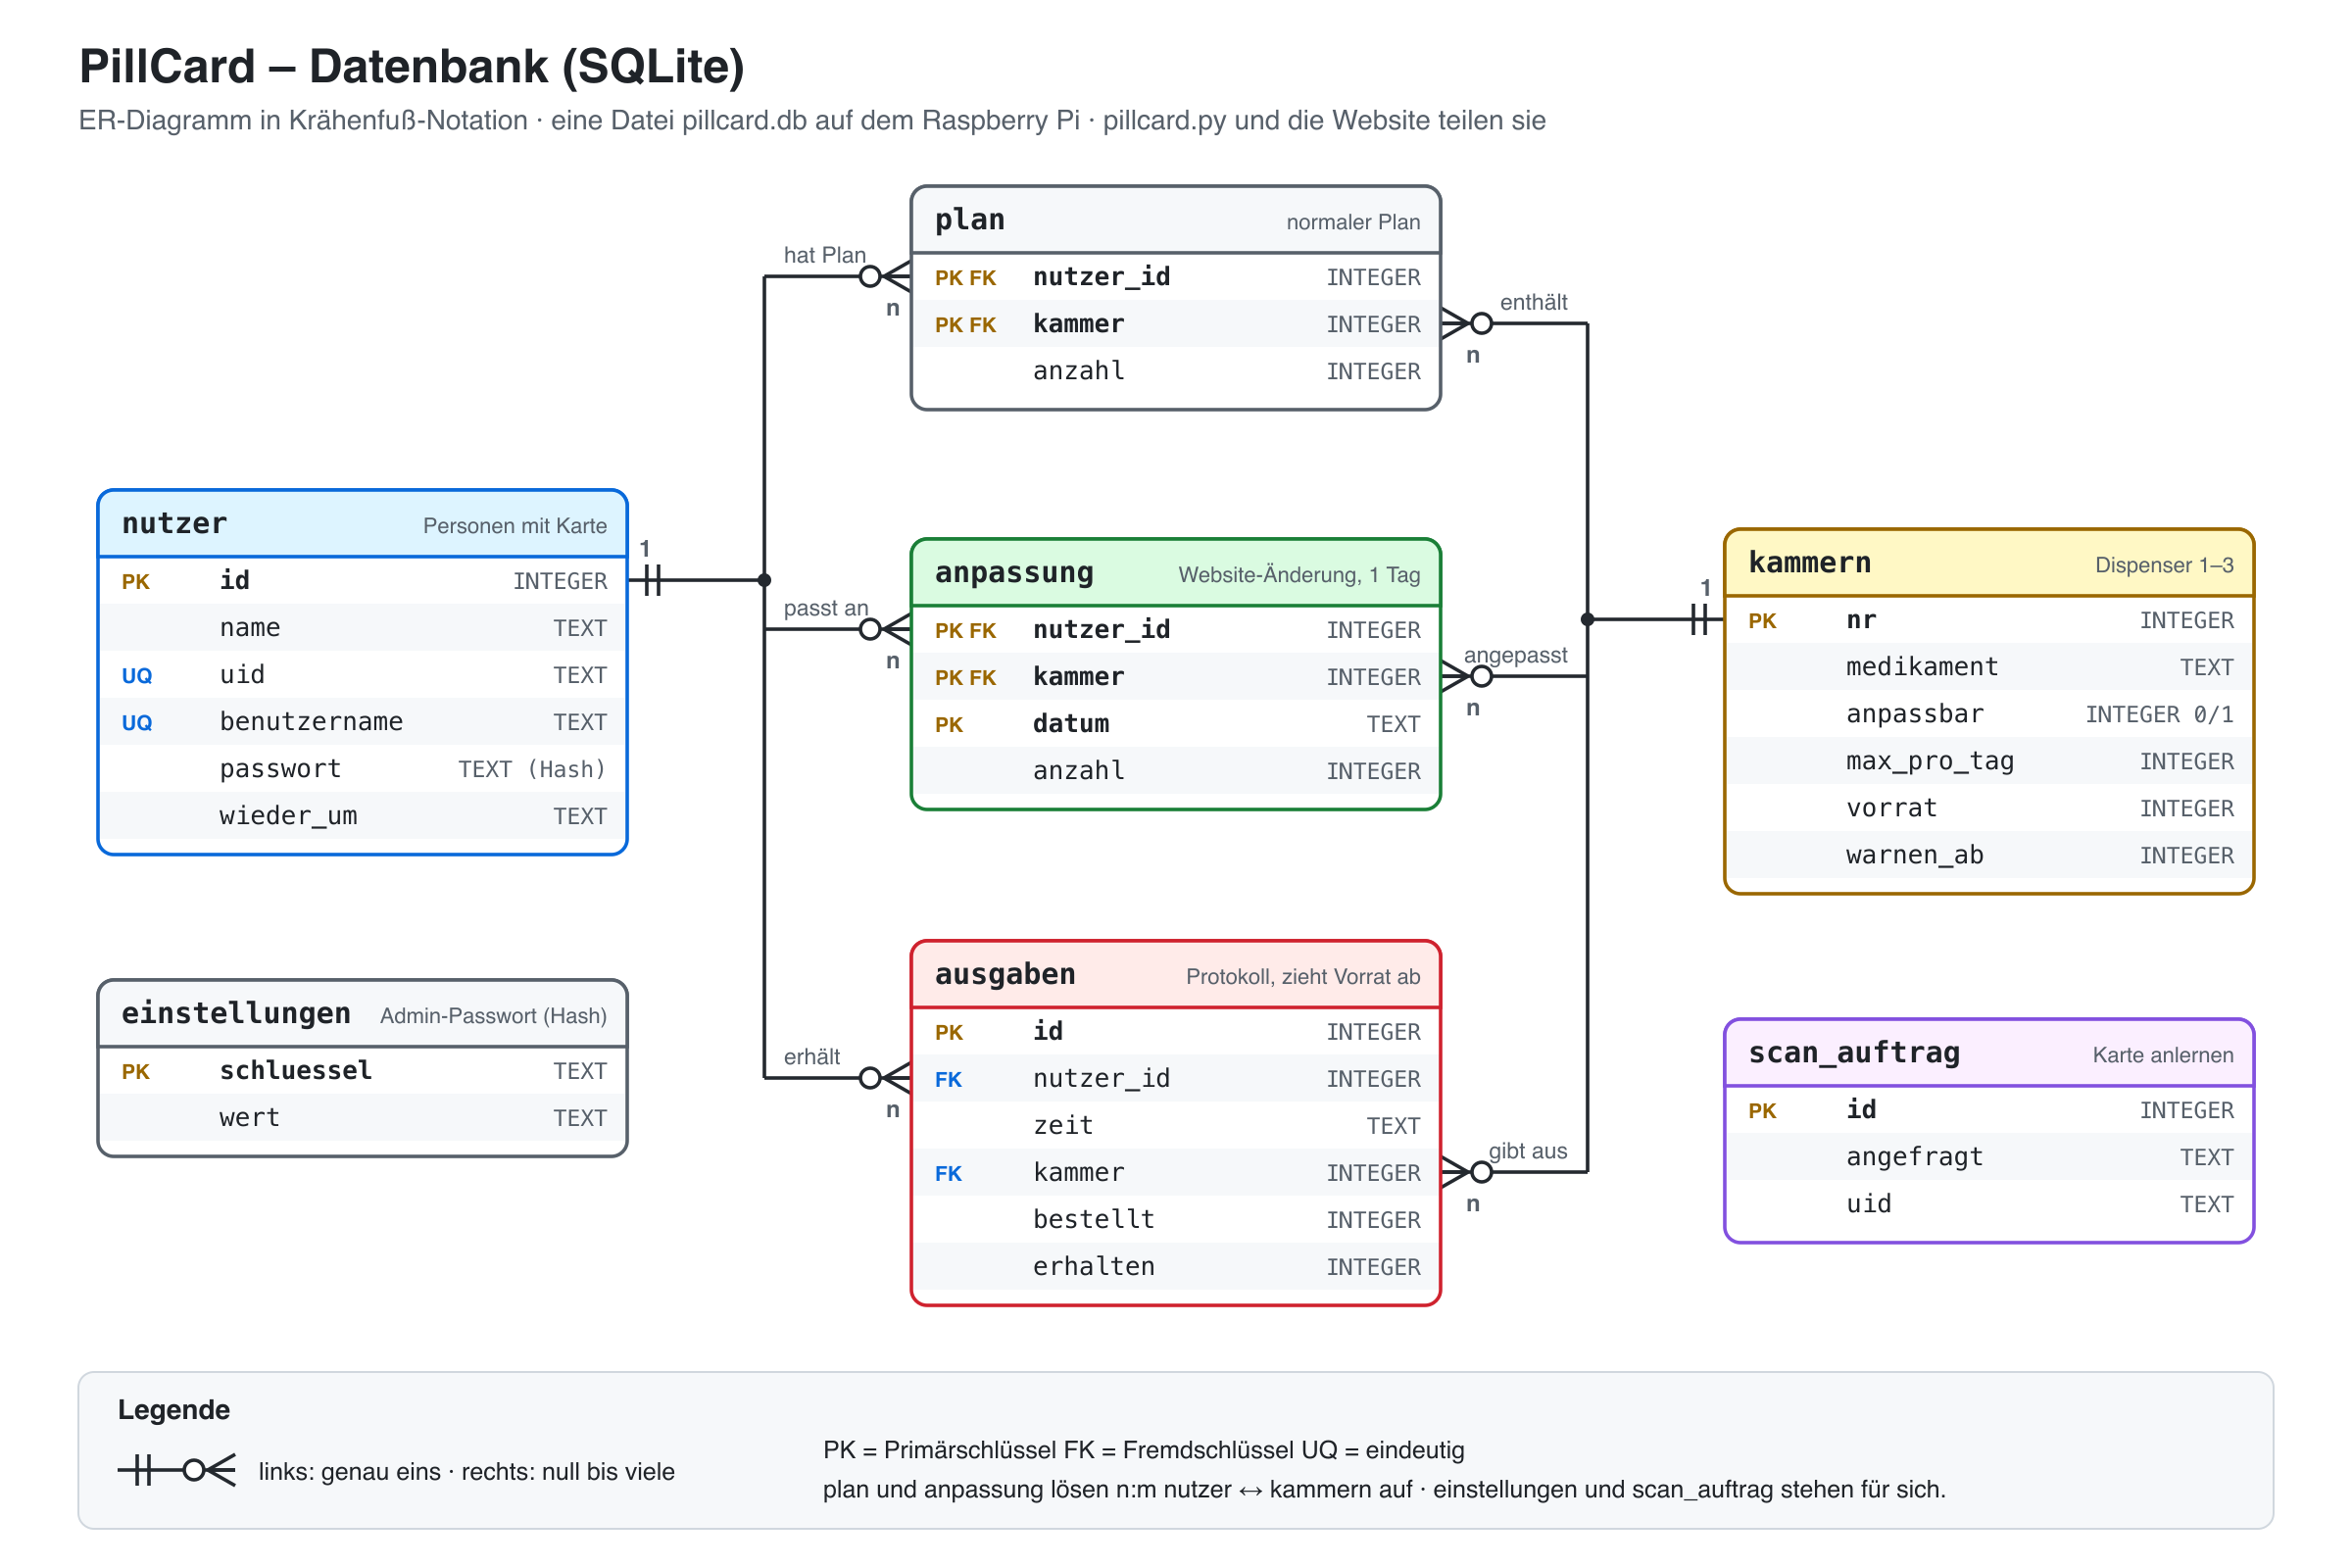
\includegraphics[width=\linewidth,height=0.55\textheight,keepaspectratio]{abbildungen/ER_Datenbank.png}
\caption{ER-Diagramm der SQLite-Datenbank. Quelle: \code{docs/ER_Datenbank.svg}.}
\label{fig:er}
\end{figure}

\paragraph{Website (\texttt{web.py}).}
Flask, ausgeliefert mit waitress, Port 8080, ohne Internetverbindung. Sie hat vier Bereiche:
\begin{itemize}
\item \textbf{Verwaltung} (\code{/admin}): Übersicht aller Personen mit Status von heute, roter Kasten
  \enquote{Heute nicht herausgekommen}, Vorrat jeder Kammer mit \enquote{reicht noch N Tage}. Neue Personen
  anlernen: Die Seite startet einen Scan, die nächste Karte am Gerät gibt nichts aus, sondern meldet ihre UID.
\item \textbf{Nutzerbereich} (\code{/}): grosse Statuskarte (\enquote{liegt bereit}, \enquote{heute erledigt},
  \enquote{nicht alle Tabletten sind herausgekommen}), was es morgen gibt, die letzten 7 Tage, Kalender
  mit Monatsbilanz und die Dosis nach Tagesform.
\item \textbf{Servo-Kalibrierung} (\code{/admin/servos}): Grundstellung in 1°- und 5°-Schritten live anfahren,
  Drehweite und Richtung pro Kammer einstellen, Probe-Ausgabe ohne Eintrag im Verlauf.
\item \textbf{Demo-Dashboard} (\code{/admin/demo}): für den Beamer, aktualisiert sich alle 2\,s und zeigt neue
  Ausgaben gross an, z.\,B.\ \enquote{Anna hat um 08:12 Uhr 4 Tabletten bekommen}.
\end{itemize}
Passwörter liegen nur als Hash in der Datenbank, Formulare haben ein Token gegen fremde Seiten. HTTPS gibt
es nicht, die Website ist nur für das Heimnetz gedacht.

\begin{figure}[H]
\centering
\foto[0.48\linewidth]{screenshot_nutzer.png}{Screenshot Nutzerbereich \enquote{Heute} mit Statuskarte}\hfill
\foto[0.48\linewidth]{screenshot_verwaltung.png}{Screenshot Verwaltung oder Demo-Dashboard}
\caption{Website: links die Sicht der Nutzerin, rechts die der Angehörigen.}
\end{figure}

\subsection{E-Rezept: neues Medikament per QR-Code}
\label{sec:erezept}

Wird eine Kammer leer, leuchtet ihre LED, und die Verwaltung bietet \enquote{E-Rezept scannen} an. Der
QR-Code eines Schweizer E-Rezepts bzw.\ eMediplans enthält die Rezeptdaten im Format CHMED16A der IG
eMediplan~\cite{chmed}, beim E-Rezept zusammen mit einem Link und einer Signatur~\cite{hin}. Das Modul
\code{pi/erezept.py} sucht im gescannten Text den CHMED-Teil, entpackt ihn (\code{CHMED16A1} = Base64 von
gzip-komprimiertem JSON) und liest Patient:in, Medikamente und Dosierung.

Den QR-Code liest der Browser aus einem Handyfoto (eingebaute Erkennung, sonst die Bibliothek
jsQR~\cite{jsqr}), alternativ tippt ein USB-QR-Scanner den Text ins Feld. Die Website schlägt die Tabletten
pro Tag (Summe aus morgens, mittags, abends, nachts) und die passende Person vor. Den Namen des Medikaments
muss man ergänzen, weil echte E-Rezepte nur GTIN oder Pharmacode enthalten. Eine Namenssuche bräuchte eine
kostenpflichtige Arzneimitteldatenbank.

\textbf{Wichtig:} Die Signatur des E-Rezepts wird nicht geprüft. Der Prototyp liest die Daten nur aus. Für die
Demo haben wir eigene Test-Codes erzeugt (\code{docs/Test-Rezepte/}, u.\,a.\ ein A4-Rezept für Anna). Das sind
keine echten Rezepte und keine echten Personendaten.

% =====================================================================
\section{Reflexion}
\label{sec:reflexion}

\subsection{Schwierigkeiten und wie wir sie gelöst haben}

\begin{table}[H]
\centering
\small
\begin{tabularx}{\linewidth}{@{}Y Y@{}}
\toprule
\textbf{Hürde} & \textbf{Lösung} \\
\midrule
RC522 meldete am Arduino Uno immer Firmware-Version 0x00, die Pins des Uno reichten ohnehin nicht. &
  Umstieg auf ESP32, später RC522 an den Pi. \\
Das LCD zeigte nur weisse Kästchen, LEDs flackerten. Verdacht: fehlende gemeinsame Masse. &
  \pruefen{Woran lag es am Ende? Masse, Pinbelegung, Kontrast-Poti?} \\
Das Beschreiben der RFID-Karten mit unserem eigenen Format hat nie geklappt. &
  Karte nur noch als ID, Plan in der Datenbank (Tabelle~\ref{tab:entscheidungen}). \\
Im Kalibrier-Sketch reagierte der Servo nach dem Speichern eines Winkels nicht mehr. &
  \pruefen{Ursache?} Später ersetzt durch die Kalibrierung über die Website. \\
Servos drehten sich ohne Ansteuerung weg, brummten am Anschlag und zogen beim Anlaufen zu viel Strom. &
  Dauerhaft ansteuern, nicht bis 0°/180° fahren, eigenes Netzteilmodul. \\
Das Mikrofon hört den Servo, und Tabletten fallen je nach Kammer erst nach bis zu 1\,s. &
  Erste 150\,ms ignorieren, Messfenster 1,8\,s, Schwelle anhand des Pegelverlaufs eingestellt. \\
Ein zweiter Ausgabeversuch bei \enquote{nicht gehört} hätte zu viele Tabletten ergeben können. &
  Kein zweiter Versuch, stattdessen ehrliche Meldung \enquote{fehlt}. \\
Nach der neuen 3D-Version stimmten Ruhelage und Drehrichtung nicht mehr. &
  Winkel und Richtung pro Kammer über die Website einstellbar. \\
Beim Öffnen der USB-Verbindung startet der ESP32 neu und verschluckt Aufträge. &
  Pi wartet auf \code{BEREIT}. \\
Eine Live-Kamera im Browser braucht HTTPS. & Foto statt Live-Bild. \\
\bottomrule
\end{tabularx}
\caption{Hürden. Quellen: \code{docs/Agent-Kontext.md}, Code-Kommentare, Git-Verlauf.}
\end{table}

\offen{Hürden bei Mechanik und Gehäuse ergänzen (Druck, Passung, Tabletten verklemmen im Magazin?, Rinne).}

\subsection{Was gut lief}

\begin{itemize}
\item \textbf{Klare Trennung über ein Textprotokoll.} Weil der ESP32 dieselben Zeilen versteht, egal ob sie vom
  Pi oder aus dem Seriellen Monitor kommen, konnten wir beide Seiten unabhängig voneinander testen.
\item \textbf{Jedes Bauteil zuerst allein.} Die kleinen Test-Sketches haben Fehler schnell eingegrenzt.
\item \textbf{Plan B war schon im Konzept.} Das Mikrofon stand im Pitch als Ausweichlösung und wurde zur
  Hauptlösung, ohne dass wir das Konzept umwerfen mussten.
\item \textbf{Vorlage statt Eigenbau beim Mechanismus.} DoseMinder hat uns das schwierigste mechanische
  Problem, das Vereinzeln, abgenommen.
\item \offen{Was lief aus eurer Sicht überraschend gut (Teamarbeit, Demo am Donnerstag, Video)?}
\end{itemize}

\subsection{Was wir gelernt haben}

\begin{itemize}
\item Komplexität lässt sich verschieben: Weil das Einstellen auf der Website liegt, kann das Gerät mit einer
  einzigen Handlung auskommen.
\item Ein Sensor misst nur, was er misst. Mikrofon und Kupferband sagen \enquote{gefallen} und
  \enquote{hochgenommen}, nicht \enquote{eingenommen}. Diese Grenze muss auch in der Oberfläche ehrlich
  stehen.
\item Hardware-Fehler sind oft Strom- und Masseprobleme, nicht Programmfehler.
\item Werte, die sich bei jedem Umbau ändern (Servo-Winkel, Mikrofonschwelle), gehören nicht fest in den Code.
\item \offen{Persönliche Lernpunkte des Teams, z.\,B.\ Löten, 3D-Druck, Arbeiten mit KI-Werkzeugen.}
\end{itemize}

\subsection{Limitationen}

Siehe Abschnitt~\ref{sec:grenzen}. Dazu kommt: Wir haben PillCard nicht mit älteren Menschen oder einer echten
WG getestet. \pruefen{Stimmt das, oder gab es Rückmeldungen, z.\,B.\ bei der Demo?} Wie zuverlässig das Mikrofon
über viele Ausgaben zählt, haben wir nicht systematisch gemessen. \offen{Falls doch: Trefferquote nennen.}

\subsection{Mögliche Erweiterungen}
\label{sec:erweiterungen}

\begin{itemize}
\item \textbf{Fernzugriff für Angehörige.} Die Website ist bisher nur im Heimnetz erreichbar. Geplant, aber nicht
  umgesetzt, ist ein Zugang über ein privates VPN (Tailscale) und HTTPS. Damit sähe das Enkelkind den Status
  auch von unterwegs, und die Live-Kamera für den QR-Code würde möglich.
\item \textbf{Benachrichtigung.} Eine Nachricht an die Angehörigen, wenn bis zu einer Uhrzeit nichts abgeholt
  wurde oder eine Tablette fehlt.
\item \textbf{Einnahmezeitpunkte.} Mehrere Ausgaben pro Tag nach Uhrzeit statt einer Tagesdosis.
\item \textbf{E-Rezept vollständig.} Signatur prüfen, Medikamentennamen über eine Arzneimitteldatenbank nachschlagen.
\item \textbf{Bessere Sensorik.} Eine Waage statt des Kupferkontakts könnte einen vollen von einem leeren Becher
  unterscheiden. Lichtschranken pro Kammer würden die Zählung unabhängig von Geräuschen machen.
\item \textbf{Sprachausgabe} über einen USB-Lautsprecher am Pi, z.\,B.\ für Menschen mit Sehschwäche.
\item \textbf{Nutzertest} mit der Zielgruppe, bevor weitere Funktionen dazukommen.
\end{itemize}

% =====================================================================
\section{Team und Aufgabenteilung}

\begin{table}[H]
\centering
\small
\begin{tabularx}{\linewidth}{@{}l Y@{}}
\toprule
\textbf{Person} & \textbf{Schwerpunkt} \\
\midrule
\stasianame & 3D-Modelle \\
\krisname & Gehäuse, Video \\
\maxname & Technik (Elektronik, ESP32- und Pi-Software, Website, Doku) und grösstenteils der Zusammenbau \\
\bottomrule
\end{tabularx}
\caption{Wer hat was gemacht.}
\end{table}

Ideenfindung, Pitch und Präsentationen haben wir gemeinsam gemacht. \pruefen{Stimmt das so?} Im Git-Verlauf
erscheinen nur Commits von Max, weil er den Code verwaltet hat. Kris (\code{codingkr1s}) und Anastasia
(\code{StasiaRic}) haben Zugriff auf das Repo.

% =====================================================================
\section{Quellen und Hilfsmittel}

\paragraph{Fremde Vorlagen.}
Magazin, Schieber, Servohalter und Rampe sind angelehnt an DoseMinder~\cite{doseminder}. Das Repo hat keine
Lizenz. Wir haben die Dateien nur als Vorlage für diesen Uni-Prototyp genutzt und geben sie nicht weiter, sie
liegen deshalb nicht in unserem Repo.

\paragraph{Bibliotheken und Werkzeuge.}
Arduino IDE mit ESP32-Core, Bibliotheken \code{LiquidCrystal} und \code{MFRC522}; Python mit Flask, waitress,
pySerial, \code{mfrc522} und \code{RPi.GPIO}; jsQR im Browser~\cite{jsqr}; FreeCAD für die 3D-Teile, Bambu
Studio zum Slicen. \offen{Software von Kris und Anastasia ergänzen.}

\paragraph{KI-Werkzeuge.}
Wir haben während des ganzen Projekts mit KI-Werkzeugen gearbeitet, vor allem mit Claude Code (Anthropic).
Es hat beim Schreiben und Debuggen von ESP32-Sketches, Pi-Programm und Website geholfen, bei der Doku
im Repo, bei den FreeCAD-Skripten für Base und Rinne und beim Entwurf dieses Berichts. Konzept,
Entscheidungen, Aufbau, Verkabelung und alle Tests an der Hardware lagen beim Team. Jeden Code haben wir am
Gerät ausprobiert, bevor er ins Repo kam. \offen{Weitere KI-Werkzeuge, z.\,B.\ für Video oder Bilder?}

\paragraph{Literatur und Quellen.}
\nocite{kurs,pillcard}
\printbibliography[heading=none]

% =====================================================================
\appendix
\section{Repository}
\label{sec:repo}

Alles zum Nachbauen liegt unter \url{https://github.com/jmax696/PillCard}:

\begin{table}[H]
\centering
\small
\begin{tabularx}{\linewidth}{@{}l Y@{}}
\toprule
\textbf{Pfad} & \textbf{Inhalt} \\
\midrule
\code{arduino-ide/PillCard_Demo/} & Sketch für den ESP32 (aktueller Stand) \\
\code{arduino-ide/*_Test/}, \code{Kammer1_RFID/} & Einzeltests der Bauteile \\
\code{pi/pillcard.py} & Kartenleser, Plan, Aufträge an den ESP32 \\
\code{pi/datenbank.py} & SQLite-Schema und Abfragen \\
\code{pi/web.py}, \code{pi/templates/}, \code{pi/static/} & Website \\
\code{pi/erezept.py} & Lesen des E-Rezept-QR-Codes (CHMED16A) \\
\code{pi/start.sh}, \code{pi/web.sh}, \code{pi/esp_flashen.sh} & Start mit Neustart-Schleife, ESP32 flashen \\
\code{docs/Verkabelung.md} & Pinbelegung, Strom, Einrichten des Pi \\
\code{docs/Schaltplan_*.svg/.png} & Schaltpläne \\
\code{docs/Datenbank.md}, \code{docs/ER_Datenbank.*} & Datenbank \\
\code{docs/Website.md} & Website und Betrieb auf dem Pi \\
\code{docs/Test-Rezepte/} & selbst erzeugte E-Rezept-QR-Codes für die Demo \\
\code{src/}, \code{lib/}, \code{include/}, \code{platformio.ini} & Frühe PlatformIO-Variante (Arduino Uno,
  Plan auf der Karte), nicht mehr benutzt \\
\bottomrule
\end{tabularx}
\end{table}

\offen{\code{README.md} und \code{REQUIREMENTS.md} beschreiben noch das Konzept vom 27.10. (Arduino Uno,
Lichtschranken). Vor der Abgabe aktualisieren oder oben einen Hinweis setzen.}
\offen{3D-Dateien (Base, Rinne, eigene Teile, ohne die DoseMinder-Originale) ins Repo legen, damit der
Prototyp nachgebaut werden kann.}

\section{Pinbelegung ESP32}
\label{sec:pins}

\begin{table}[H]
\centering
\small
\begin{tabularx}{\linewidth}{@{}l l Y@{}}
\toprule
\textbf{Bauteil} & \textbf{ESP32} & \textbf{Hinweis} \\
\midrule
LCD RS / E & IO22 / IO21 & R/W fest an GND \\
LCD D4 / D5 / D6 / D7 & IO32 / IO33 / IO14 / IO15 & 4-Bit-Modus, V0 am Poti \\
Servo Kammer 1 / 2 / 3 & IO25 / IO26 / IO27 & Strom vom Netzteilmodul \\
LED grün / rot & IO16 / IO17 & je über 100\,$\Omega$ \\
Leer-LED Kammer 1 / 2 / 3 & IO18 / IO19 / IO23 & je über 100\,$\Omega$ \\
Mikrofon (Signal) & IO34 & Versorgung 3,3\,V \\
Becherkontakt & IO13 & 1\,k$\Omega$ in Reihe, 10\,k$\Omega$ an 3,3\,V, 100\,nF an GND \\
Raspberry Pi & USB & Strom und Textprotokoll, 115200 Baud \\
\bottomrule
\end{tabularx}
\end{table}

RC522 am Raspberry Pi (Stiftnummern der 40-poligen Leiste): SDA Pin~24, SCK Pin~23, MOSI Pin~19, MISO Pin~21,
RST Pin~22, GND Pin~20, 3,3\,V Pin~17.

% =====================================================================
\newpage
\section*{Eigenständigkeitserklärung}
\addcontentsline{toc}{section}{Eigenständigkeitserklärung}

\small
Text nach Erlass II.A.05 der Universität St.Gallen (Stand 1.~Februar 2023). Jedes Teammitglied gibt die
Erklärung für sich ab.
\pruefen{Klären, ob bei Gruppenarbeiten \enquote{wir} statt \enquote{ich} verwendet werden darf.}

\begin{quote}
„Ich erkläre hiermit,
\begin{itemize}
\item dass ich die vorliegende Arbeit eigenständig verfasst habe,
\item dass ich die Arbeit nur unter Verwendung der im Verzeichnis angegebenen Hilfsmittel verfasst habe;
\item dass alle mit Hilfsmitteln erbrachten Teile der Arbeit präzise deklariert wurden;
\item dass ich sämtliche verwendeten Quellen erwähnt und gemäss gängigen wissenschaftlichen Zitierregeln korrekt
  zitiert habe;
\item dass ich sämtliche immateriellen Rechte an von mir allfällig verwendeten Materialien wie Bilder oder Grafiken
  erworben habe oder dass diese Materialien von mir selbst erstellt wurden;
\item dass das Thema, die Arbeit oder Teile davon nicht bereits Gegenstand eines Leistungsnachweises einer anderen
  Veranstaltung oder Kurses waren, sofern dies nicht ausdrücklich mit der Referentin oder dem Referenten im Voraus
  vereinbart wurde und in der Arbeit ausgewiesen wird;
\item dass ich mir über die rechtlichen Bestimmungen zur Publikation und Weitergabe von Teilen oder der ganzen
  Arbeit bewusst bin und ich diese entsprechend einhalte;
\item dass ich mir bewusst bin, dass meine Arbeit elektronisch auf Plagiate und auf Drittautorschaft menschlichen
  oder technischen Ursprungs überprüft werden kann und ich hiermit der Universität St.Gallen laut Prüfungsordnung
  das Urheberrecht soweit einräume, wie es für die Verwaltungshandlungen notwendig ist;
\item dass ich mir bewusst bin, dass die Universität einen Verstoss gegen diese Eigenständigkeitserklärung verfolgt
  und dass daraus disziplinarische wie auch strafrechtliche Folgen resultieren können, welche zum Ausschluss von
  der Universität resp.\ zur Titelaberkennung führen können.“
\end{itemize}
\end{quote}

Mit Einreichung der schriftlichen Arbeit stimme ich mit konkludentem Handeln zu, die Eigenständigkeitserklärung
abzugeben, diese gelesen sowie verstanden zu haben und, dass sie der Wahrheit entspricht.

\normalsize
\vspace{2em}
\begin{tabularx}{\linewidth}{@{}X X X@{}}
St.Gallen, 20.11.2026 & St.Gallen, 20.11.2026 & St.Gallen, 20.11.2026 \\[2.5em]
\rule{0.9\linewidth}{0.4pt} & \rule{0.9\linewidth}{0.4pt} & \rule{0.9\linewidth}{0.4pt} \\
Max Jäckle & Anastasia \offen{Nachname} & Kris \offen{Nachname} \\
\end{tabularx}

\end{document}
